\iffalse
    \author{EE24BTECH11061}
    \section{ce}
    \chapter{2020}
 \fi
%\begin{enumerate}
\item The area of an ellipse represented by an equation $\frac{x^2}{a^2} + \frac{y^2}{b^2} = 1$ is
\begin{multicols}{2}
    \begin{enumerate}
        \item $\frac{\pi a b}{4}$
        \item $\frac{\pi a b}{2}$
        \item $\pi a b$
        \item $\frac{4 \pi a b}{3}$
    \end{enumerate}
\end{multicols}

\item Consider the planar truss shown in the figure \textit{(not drawn to scale)}
% myy ownnn codeeeee T_T
\centering
\begin{tikzpicture}[H]
    \draw[thick] (0,0) -- (6,0);
    \draw[thick] (0,0) -- (0,-2);
    \draw[thick] (0,-2) -- (6,0);
    \draw[thick] (0,-2) -- (2,0);
    \draw[thick] (2,0) -- (2,-1.33);
    \draw[thick] (2,-1.33) -- (4,0);
    \draw[thick] (4,0) -- (4,-0.66);

    \draw[thick, <->] (0,0.3) -- (2,0.3);
    \draw[thick, <->] (2,0.3) -- (4,0.3);
    \draw[thick, <->] (4,0.3) -- (6,0.3);
    \draw[thick, <->] (-1.2,0) -- (-1.2, -2);

    \node at (1,0.5) {$L$};
    \node at (3,0.5) {$L$};
    \node at (5,0.5) {$L$};
    \node at (-1,-1) {$L$};

    \node at (0,0) [circle, draw = black, line width = 0.3mm, fill = white, inner sep = 2 pt]{};
    \node at (2,0) [circle, draw = black, line width = 0.3mm, fill = white, inner sep = 2 pt]{};
    \node at (4,0) [circle, draw = black, line width = 0.3mm, fill = white, inner sep = 2 pt]{};
    \node at (6,0) [circle, draw = black, line width = 0.3mm, fill = white, inner sep = 2 pt]{};
    \node at (4,-0.66) [circle, draw = black, line width = 0.3mm, fill = white, inner sep = 2 pt]{};
    \node at (2,-1.33) [circle, draw = black, line width = 0.3mm, fill = white, inner sep = 2 pt]{};
    \node at (0,-2) [circle, draw = black, line width = 0.3mm, fill = white, inner sep = 2 pt]{};

    \draw[thick] (-0.1,0.05) -- (-0.4,-0.4) -- (-0.4,0.4) -- (-0.1, -0.05) -- cycle;
    \draw[thick] (-0.1,-2.05) -- (-0.4,-1.6) -- (-0.4,-2.4) -- (-0.1, -1.95) -- cycle;

    \draw[thick, ->] (2,-1.40) -- (2,-2.2);
    \node at (2.3,-2) {$P$};
\end{tikzpicture}\\
Neglecting self-weight of the members, the number of zero-force members in the truss under the action of the load $P$, is
\begin{multicols}{2}
    \begin{enumerate}
        \item 6
        \item 7
        \item 8
        \item 9
    \end{enumerate}
\end{multicols}
    
\item A reinforcing steel bar, partially embedded in concrete, is subjected to a tensile force $P$, The figure that approximately represents the distribution of the magnitude of bond stress (represented as hatched region), along the embedded length of the bar, is
\begin{multicols}{2}
    \begin{enumerate}
        \item 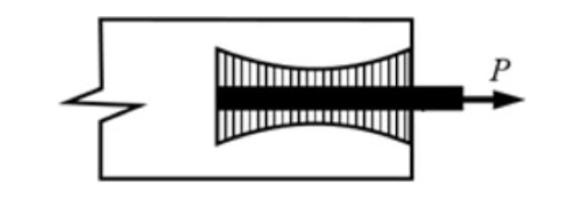
\includegraphics[width=0.5\linewidth]{GATE-yearwise/2020/figs/fig_a.png}
        \item 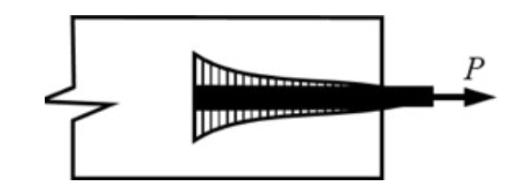
\includegraphics[width=0.5\linewidth]{GATE-yearwise/2020/figs/fig_b.png}
        \item 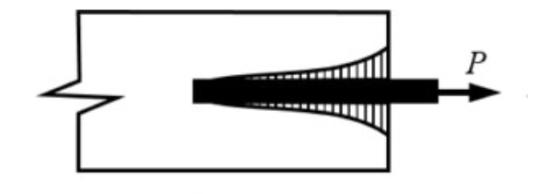
\includegraphics[width=0.5\linewidth]{GATE-yearwise/2020/figs/fig_c.png}
        \item 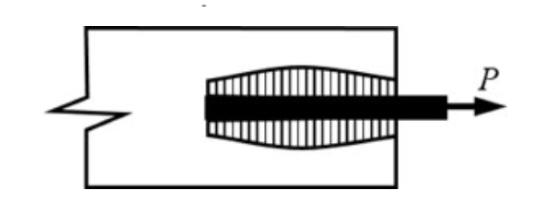
\includegraphics[width=0.5\linewidth]{GATE-yearwise/2020/figs/fig_d.png}
    \end{enumerate}
\end{multicols}

\item In a two-dimensional stress analysis, the state of stress at a point $P$ is
\begin{align*}
    \myvec{\sigma} = \myvec{\sigma_{xx} & \tau_{xy} \\ \tau_{xy} & \sigma_{yy}}
\end{align*}
The necessary and sufficient condition for existence of the state of pure shear at the point $P$, is
\begin{multicols}{2}
    \begin{enumerate}
        \item $\sigma_{xx} \sigma_{yy} - \tau^2_{xy} = 0$
        \item $\tau_{xy} = 0$
        \item $\sigma_{xx} + \sigma_{yy} = 0$
        \item $\brak{\sigma_{xx} - \sigma_{yy}}^2 + 4 \tau^2_{xy} = 0$
    \end{enumerate}
\end{multicols}

\item During the process of hydration of cement, due to increase in Dicalcium Silicate $\brak{\text{C}_2\text{S}}$ content in cement clinker, the heat of hydration
\begin{multicols}{2}
    \begin{enumerate}
        \item increases
        \item decrease
        \item initially decreases and then increase
        \item does not change
    \end{enumerate}
\end{multicols}

\item The Los Angeles test for stone aggregates is used to examine
\begin{multicols}{2}
    \begin{enumerate}
        \item abrasion resistance
        \item crushing strength
        \item soundness
        \item specific gravity
    \end{enumerate}
\end{multicols}

\item Which one of the following statements is \textbf{NOT} correct?
\begin{multicols}{2}
    \begin{enumerate}
        \item A clay deposit with a liquidity index greater than unity is in a state of plastic consistency.
        \item The cohesion of normally consolidated clay is zero when triaxial test is conducted under consolidated undrained condition.
        \item The ultimate bearing capacity of a strip foundation supported on the surface of sandy soil increases in direct proportion to the width of footing.
        \item In case of a point load, Boussinesq's equation predicts higher value of vertical stress at a point directly beneath the load as compared to Westergaard's equation.
    \end{enumerate}
\end{multicols}

\item In a soil investigation work at a site, Standard Penetration Test (SPT) was conducted at every 1.5 m  interval up to 30 m depth. At 3 m depth, the observed number of hammer blows for three successive 150 m penetrations were 8, 6 and 9, respectively. The SPT N-value at 3 m depth, is
\begin{multicols}{2}
    \begin{enumerate}
        \item 23
        \item 17
        \item 15
        \item 14
    \end{enumerate}
\end{multicols}

\item Velocity of flow is proportional to the first power of hydraulic gradient in Darcy's law. This law is applicable to
\begin{multicols}{2}
    \begin{enumerate}
        \item laminar flow in porous media
        \item transitional flow in porous media
        \item turbulent flow in porous media
        \item laminar as well as turbulent flow in porous media
    \end{enumerate}
\end{multicols}

\item A body flowing in a liquid is in a stable state of equilibrium is its
\begin{multicols}{2}
    \begin{enumerate}
        \item metacentre lies above its centre of gravity
        \item metacentre lies below its centre of gravity
        \item metacentre coincides with its centre of gravity
        \item centre of gravity is below its centre of buoyancy
    \end{enumerate}
\end{multicols}

\item Uniform flow with velocity $U$ makes an angle $\theta$ with the y-axis, as shown in the figure 
%figure
\begin{figure}[h!]
    \centering
    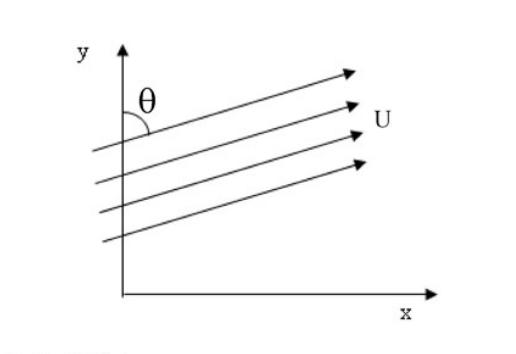
\includegraphics[width=0.5\linewidth]{GATE-yearwise/2020/figs/graph.png}
    \label{fig:enter-label}
\end{figure}\\
The velocity potential $\brak{\phi}$, is
\begin{multicols}{2}
    \begin{enumerate}
        \item $\pm U \brak{x \sin{\theta} + y \cos{\theta}}$
        \item $\pm U \brak{y \sin{\theta} - x \cos{\theta}}$
        \item $\pm U \brak{x \sin{\theta} - y \cos{\theta}}$
        \item $\pm U \brak{y \sin{\theta} + x \cos{\theta}}$
    \end{enumerate}
\end{multicols}

\item The data for an agricultural field for a specific month are given below:
\begin{align*}
    \text{Pan Evaporation} & = 100 \, \text{mm} \\
    \text{Effective Rainfall} & = 20 \, \text{mm} \, \text{(after deducting losses due to runoff and deep percolation)} \\
    \text{Crop Coefficient} & = 0.4 \\
    \text{Irrigation Efficiency} & = 0.5
\end{align*}
The amount of irrigation water (in mm) to be applied to the field in that month, is
\begin{multicols}{2}
    \begin{enumerate}
        \item 0
        \item 20
        \item 40
        \item 80
    \end{enumerate}
\end{multicols}

\item During chlorination process, aqueous (aq) chlorine reacts rapidly with water to form Cl$^{-}$, HOCl, and H$^{+}$ as shown below
\begin{align*}
    \text{Cl}_2 \brak{aq} + \text{H}_2 \text{O} \rightleftharpoons \text{HOCl} + \text{Cl}^{-} + \text{H}^{+}
\end{align*}
The most active disinfectant in the chlorination process from amongst the following, is
\begin{multicols}{2}
    \begin{enumerate}
        \item H$^{+}$
        \item HOCl
        \item Cl$^{-}$
        \item H$_2$O
    \end{enumerate}
\end{multicols}
%\end{enumerate}